\newcommand{\A}{\mathbb{A}}
\newcommand{\D}{\mathbb{D}}
\newcommand{\Z}{\mathbb{Z}}
\newcommand{\R}{\mathbb{R}}
\newcommand{\C}{\mathbb{C}}
\newcommand{\T}{\mathbb{T}}
\newcommand{\N}{\mathbb{N}}
\newcommand{\s}{\mathbb{S}}
\newcommand{\tu}{\tilde{U}}
\newcommand{\F}{\mathcal{F}}
\newcommand{\fall}{\;\forall\;}
\newcommand{\exst}{\;\exists\;}
\newcommand{\nexst}{\;\not\exists\;}
\newcommand{\br}{\par\vspace{10pt}}
\newcommand{\Ch}{C_n(X)}
\newcommand{\ch}{C_{n-1}(X)}
\newcommand{\dx}{\Delta_n(X)}
\newcommand{\ddx}{\Delta_{n-1}(X)}

\providecommand{\comm}{\todo[inline, color=SpringGreen!40]}
\providecommand{\duda}{\todo[inline, color=Apricot!40]}

\documentclass{cmat-monografia}

\usepackage{lipsum}
\usepackage{amssymb}
\usepackage{todonotes}
\usepackage[dvipsnames]{xcolor}
\usepackage[figurename=Imagen]{caption}

\theoremstyle{definition}
\newtheorem{df}{Definición}[chapter]
\newtheorem{obs}[df]{Observación}
\newtheorem{ex}[df]{Ejemplo}

\theoremstyle{plain}
\newtheorem{prop}[df]{Proposición}
\newtheorem{teo}[df]{Teorema}
\newtheorem{cor}[df]{Corolario}
\newtheorem{lema}[df]{Lema}

\title{Elementos de la Matemática}

\author{Nicolas Bourbaki}

\subtitle{Topología}

\director{André Weil}

\codirector{Lauren Schwartz}

\inst{ENS}

\coinst{École Polytechnique}

\parindent 0pt


\begin{document}

\maketitle
\begin{abstract}

\vspace{10pt}\par

Un encaje de $S^1$ en $S^2$ es una función $f:S^1\to S^2$ inyectiva y continua. Una función así es un homeomorfismo sobre su imagen, y por lo tanto $f(S^1)$ es una curva cerrada simple $\gamma$. ¿Qué sabemos sobre $\gamma$? Desde hace 150 años se sabe que $\gamma$ separa a $S^2$ en dos componentes conexas. Hace 100 años se probó que además existe un homeomorfismo $h:S^2\to S^2$ que manda $\gamma$ en $S^1$, lo que tiene como consecuencia que las componentes conexas de $\gamma^c$ tienen $\pi_1=0$. \par
\vspace{10pt}
\comm{qué sabemos sobre $ \gamma$ me parece muy general y no sé q cosas más "sabemos" sobre $\gamma$ q se me escapan}

¿Qué pasa en general con encajes de $f:S^{n-1}\to S^n$? Desde hace 100 años sabemos que $f(S^{n-1})^c$ tiene dos componentes conexas. Sin embargo, en estos casos no necesariamente existe un homeomorfismo $h:S^n\to S^n$ que mande $f(S^n)$ al encaje usual de $S^{n-1}\subset S^n$.\br

Estos dos útlimos resultados se probarán en esta monografía. Para el primero se introducirá al lector a la teoría de homología singular y se probarán algunos resultados sobre la misma. Para probar que el homeomorfismo $f$ no necesariamente se extiende a todo $S^n$, darán dos ejemplos de 2-esferas $S$ encajadas en $R^3$ con $\pi_1(S^c)\neq\varnothing$. Además veremos que los $\pi_1(S)$ serán ejemplos de grupos no triviales cuyo abelianizado es trivial.\br

Después veremos cositas de límites inversos y atractores de sistemas dinámicos.\comm{escribir xd}

\end{abstract}

\chapter{Preliminares}

En general, notamos $S^n := \{x\in\R^n : \|x\|=1\}$, y decimos que una $n-$esfera es un espacio topológico $S$ tal que existe un homeomorfismo $h:S\to S^n$.\br

\chapter{Homología y teorema de Jordan}

En esta sección introduciremos al lector a la teoría de homología singular. El objetivo será probar que una $(n-1)$-esfera separa $\R^n$ en dos componentes conexas, y que estas componentes conexas tienen la misma homología de un punto. \br

Para empezar, definiremos lo que es un $n$-símplice:

\begin{df} Un $n$-símplice es el menor conjunto convexo de $\R^{m}\; (m\geq n)$ que contiene $n+1$ puntos $v_0,\dots,v_n$, tales que $v_1-v_0$, $v_2-v_0$, $\dots$, $v_n-v_0$ son linealmente independientes. Llamaremos vértices a estos $v_i$.\end{df}\br

En general, dado un $n$-símplice, vamos a darle un orden a sus vértices, y notaremos al símplice $[v_0,v_1,\dots,v_n]$ de acuerdo con este orden. \br

\begin{df}
Un orden en los vértices nos induce un orden en la restricción a un subconjunto de esos vértices. Haremos uso de la siguiente notación:
$$[v_0,\dots,\hat{v_i},\dots,v_n]:=[v_0,\dots,v_{i-1},v_{i+1},\dots,v_n]$$ 
Esta es una forma de notar el $(n-1)$-símplice obtenido al sacar $v_i$ del conjunto de vértices de $[v_0,\dots,v_n]$ y tomar el menor conjunto convexo que contiene a los vértices restantes. \br

Diremos que $[v_0,\dots,\hat{v_i},\dots,v_n]$ es una cara de $[v_0,\dots,v_n]$.\br

Llamaremos aristas a los $2$-símplices con vértices $v_i, v_j\in\{v_0,\dots,v_n\}$. Estas también heredan el orden de $[v_0,\dots,v_n]$, y por lo tanto las notamos $[v_i,v_j]$ si $i<j$.
\end{df}

% Al definirlo así, implícitamente le estamos dando a los vértices de $[v_0,\dots,\hat{v_i},\dots,v_n]$ el orden heredado de restringir el orden de $[v_0,\dots,v_n]$ al nuevo conjunto de vértices. \br

Un ejemplo de $3$-símplice es un tetraedro en $\R^3$, un $2$-símplice es un triángulo en $\R^2$, un $1$-símplice es un intervalo en $\R$, y un $0$-símplice es un punto.\br


\begin{figure}[h!]
    \centering
    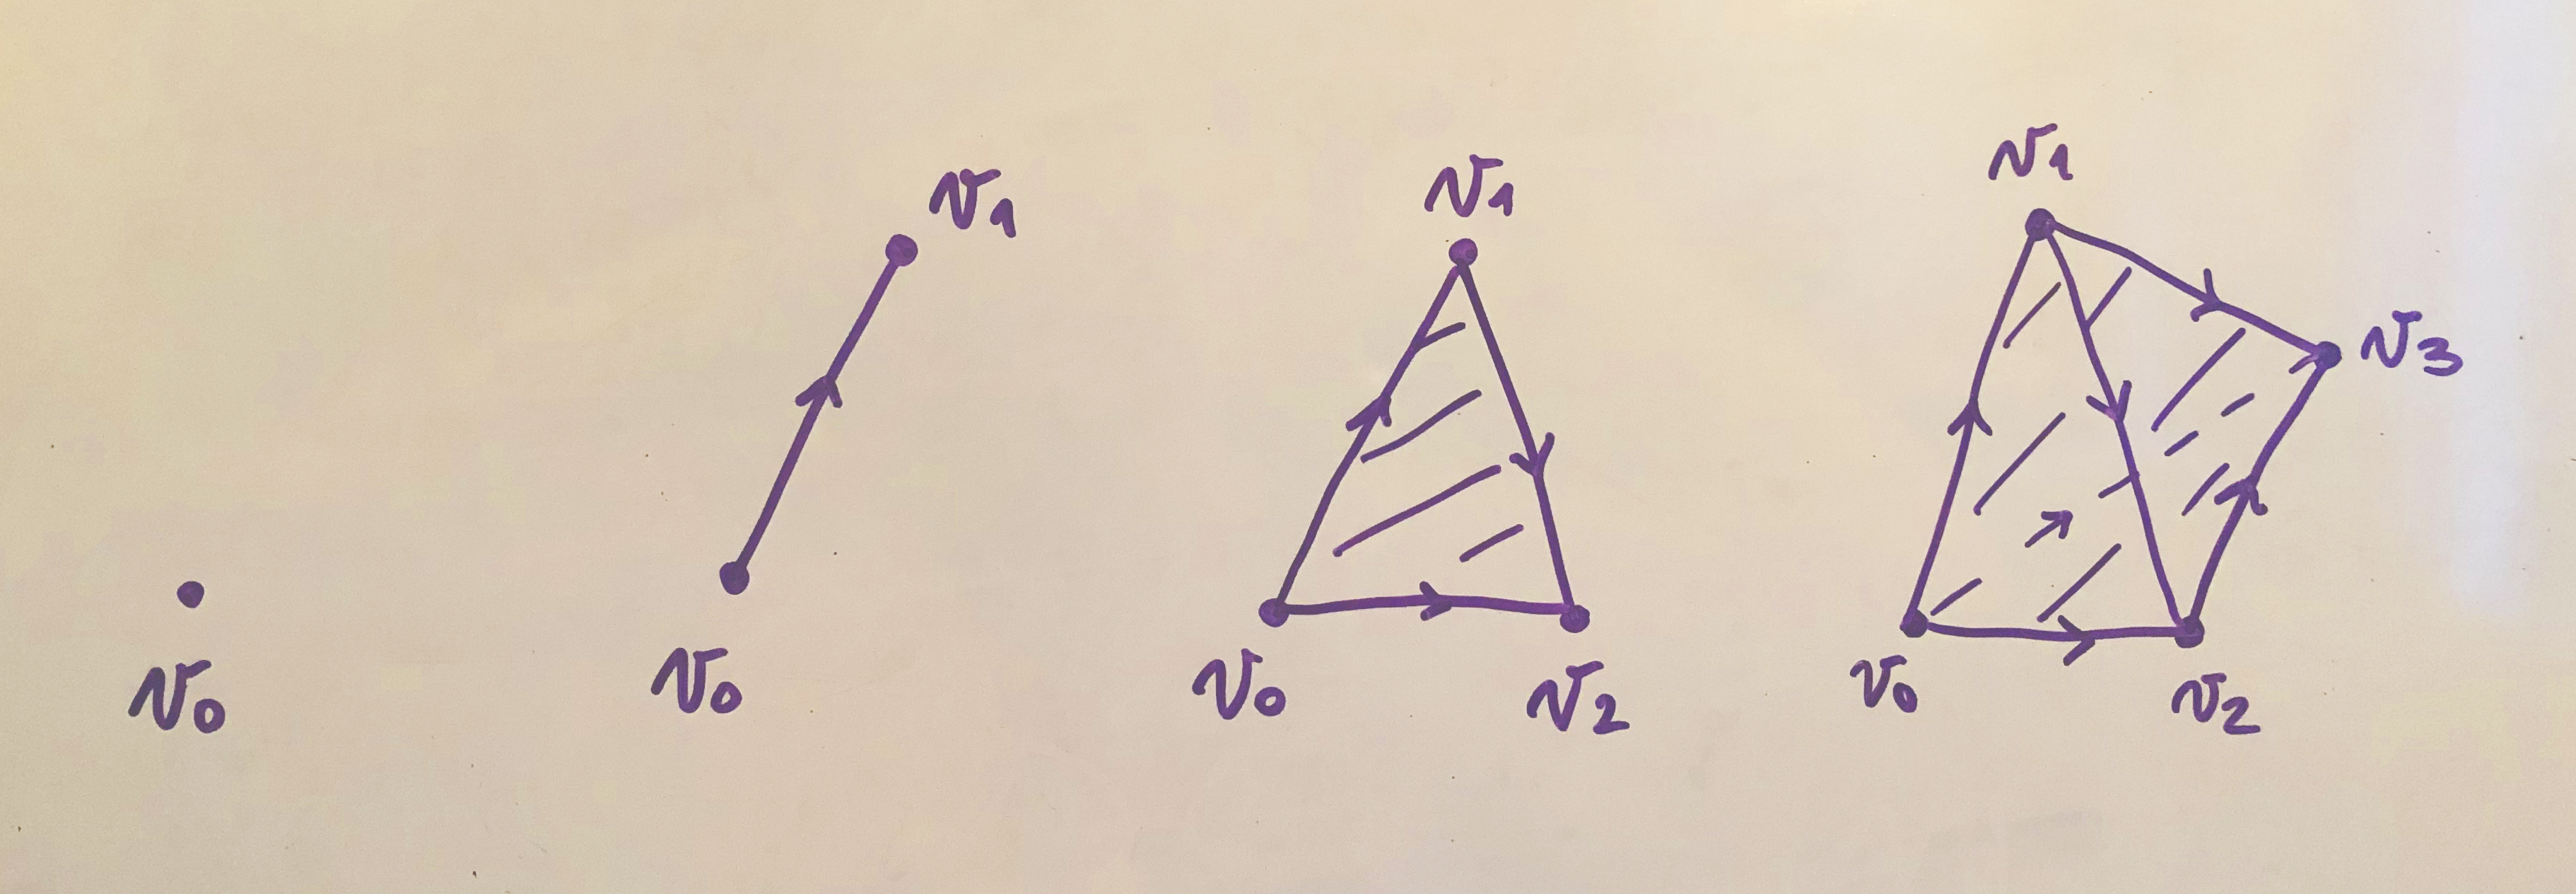
\includegraphics[width=0.5\linewidth]{img mono/simplices.png}
    \caption{$n$-símplices con las orientaciones de sus aristas, $n\in\{0,1,2,3\}$}
    \label{fig:placeholder}
\end{figure}

\comm{las imágenes no son finales, eventualmente las voy a hacer en digital}

\begin{df}
Llamaremos $n$-símplice estándar al conjunto $$\Delta^n := \Bigl\{(x_0,\dots,x_n)\in\R^{n+1} : x_i\geq 0\text{ para todo } i, \;\sum\limits_{i=0}^nx_i=1\Bigr\}$$
\end{df}

Los vértices de este $n$-símplice son los que conforman la base canónica de $\R^{n+1}$. Si notamos a estos puntos $e_1,\dots,e_{n+1}$, otra forma de escribir este conjunto es $$\Delta^n=[e_1,\dots,e_{n+1}] \subset \R^{n+1}$$\br

Para $n=2$, el $2$-símplice estándar $\Delta^2$ es el triángulo en $\R^3$ con vértices $(1,0,0)$, $(0,1,0)$ y $ (0,0,1)$. Con $n=1$, el $1$-símplice estándar es el segmento que va de $(1,0)$ a $(0,1)$ en $\R^2$. \br

\begin{figure}[h!]
    \centering
    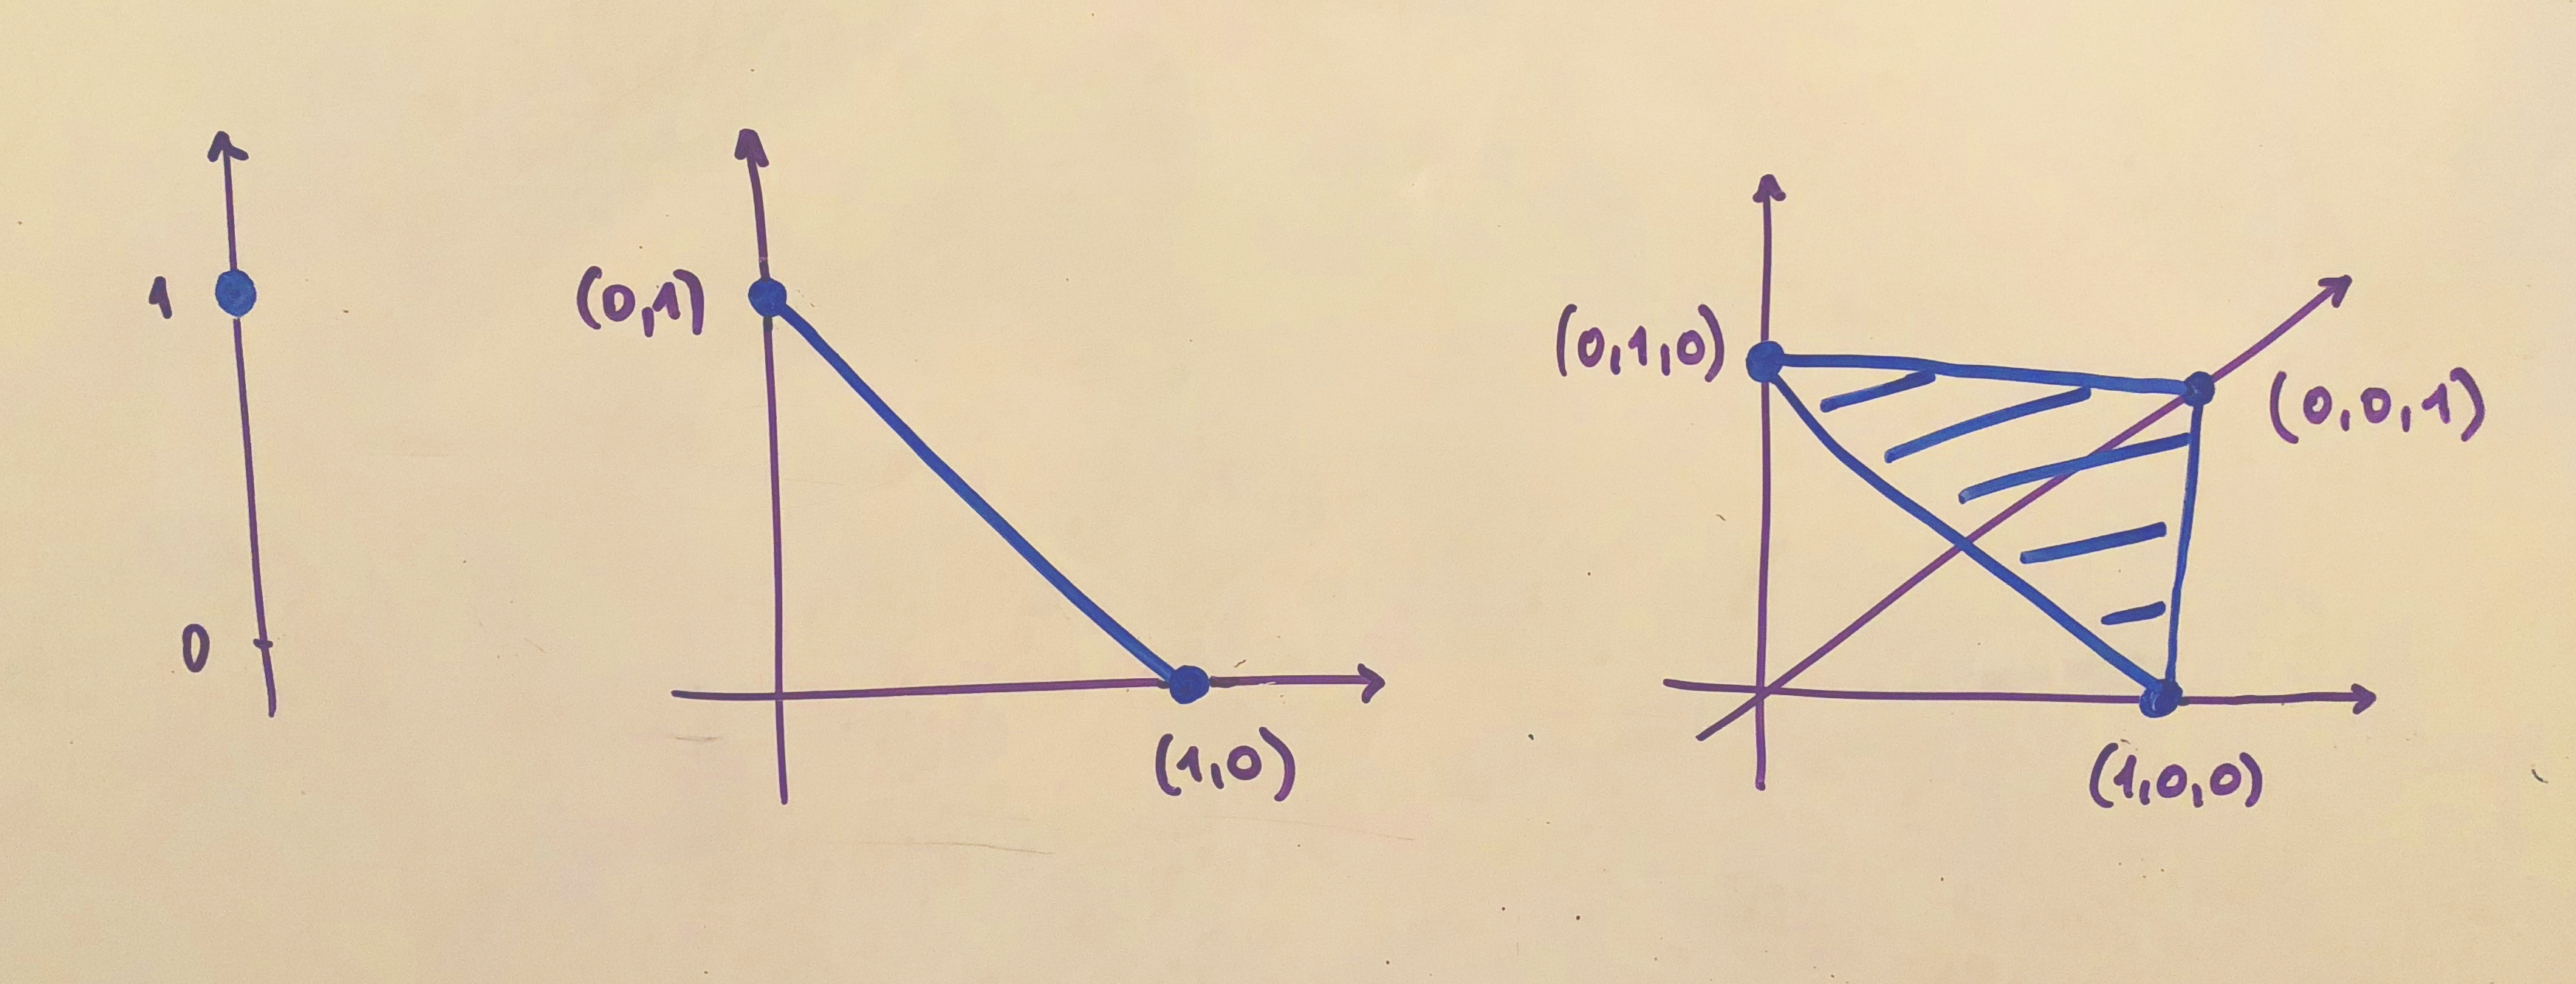
\includegraphics[width=0.5\linewidth]{img mono/simplices estandar.png}
    \caption{$n$-símplices estándar, $n\in\{0,1,2\}$}
\end{figure}

\begin{df}
Dado un $n$-símplice $[v_0,\dots,v_n]$,  la función $h:\Delta^n\to [v_0,\dots,v_n]$ dada por $$h(x_0,\dots,x_n)=\sum\limits_{i=0}^n x_i v_i$$ es un homeomorfismo lineal que preserva el orden de las aristas. Llamaremos a esta función el homeomorfismo canónico.
\end{df}\br

La función $h$ es lineal y manda los elementos $e_0,\dots,e_n$ de la base canónica de $\R^{n+1}$ a $v_0,\dots, v_n$ respectivamente, por lo tanto su imagen es el $n$-símplice $[v_0,\dots,v_n]$ y el orden de las aristas se mantiene.\br

Antes de entrar en la definición de homología singular, vamos a definir la homología simplicial, que nos va a dar una imagen de las intuiciones que en la homología singular se ven más ofuscadas a cambio de obtener una teoría menos rígida y más limpia para trabajar.  \br

Para empezar, vamos a definir lo que será una estructura de $\Delta$-complejo para un espacio topológico cualquiera. Esto va a ser el análogo en dimensión $n$ de triangular nuestro espacio con $2$-símplices.\br


\begin{df}
    Una estructura de $\Delta$-complejo para un espacio topológico $X$ es una familia de funciones continuas $\sigma_\alpha:\Delta^{n_\alpha}\to X$ que cumplen:

    \begin{enumerate}
        \item Las $\sigma_\alpha$ son inyectivas al restringirlas a $Int(\Delta^{n_\alpha})$, y dado cualquier $x\in X$, existe algún $\alpha$ tal que $x$ está en la imagen de $Int(\Delta^{n_\alpha})$ por $\sigma_\alpha$.
        
        \item Si restringimos cualquier $\sigma_\alpha$ a una cara de $\Delta^{n_\alpha}$, esa restricción va a ser equivalente a otro mapa de la familia $\sigma_\beta:\Delta^{n_\alpha-1}\to X$, identificando la cara de $\Delta^{n_\alpha}$ con $\Delta^{n_\alpha-1}$ mediante el homeomorfismo canónico.

        \item Un conjunto $U\subset X$ es abierto $\iff$ $\sigma_\alpha^{-1}(U)$ es abierto para todo $\alpha$.
    \end{enumerate}\br

    En el punto $(2)$, la equivalencia es en el siguiente sentido: \br

    Dada $\sigma_\alpha:\Delta^{n_\alpha}\to X$, notamos $\hat{\Delta}^{n_\alpha}$ a una cara de $\Delta^{n_\alpha}$. Consideramos $h:\Delta^{n_\alpha -1}\to\hat{\Delta}^{n_\alpha}$ el homeomorfismo canónico que manda el $\{n_\alpha -1\}$-símplice estándar a $\hat{\Delta}^{n_\alpha}$. Lo que nos dice este punto es que existe una función $\sigma_\beta:\Delta^{n_\alpha -1}\to X$ en la familia que cumple $\sigma_\beta=\sigma_\alpha\circ h$.
\end{df}

Las condiciones $(1)$ y $(3)$ nos dicen que las funciones $\sigma_\alpha$ restrictas a $Int(\Delta^{n_\alpha})$ son homeomorfismos sobre su imagen. Esta estructura nos permite ver a $X$ como cociente de símplices, identificando las caras necesarias mediante homeomorfismos canónicos.\br

\comm{capaz decir algo más acá y poner una imagen, obs sobre hff}

\begin{df}
    Dada una estructura de $\Delta$-complejo para un espacio $X$, definimos $\dx$ como el grupo abeliano libre generado por los $\{\sigma_\alpha:\Delta^{n_\alpha}\to X \; | \; n_\alpha=n\}$. Es decir, los elementos de $\dx$, a los que llamaremos $n$-cadenas, son sumas formales finitas $\sum_{i=1}^{N} k_i\sigma_i$, con $k_i\in\N$.
\end{df}

Observar que el borde de un $n$-símplice $\Delta^n$ es la unión de sus $n+1$ caras, que notaremos $\partial\Delta^n$. \br
\begin{df}
Vamos a definir un homomorfismo de grupos $\partial_n:\dx\to\ddx$ al que llamaremos mapa borde, lo definiremos mediante su valor en los generadores de $\dx$, es decir, las funciones $\sigma_\alpha :\dx\to X$. 

Dada $\sigma_\alpha:\dx\to X$, notamos $\Delta^n = [v_0,\dots,v_n]$ y definimos $$\partial(\sigma_\alpha):=\sum\limits_{i=0}^{k}(-1)^i \sigma|_{[v_0,\dots,\hat{v_i},\dots v_n]}$$ 
\end{df}

\comm{explicar intuición del $(-1)^i$}
% La idea atrás del $(-1)^i$ es orientar

\begin{lema}
La composición $\partial_{n-1}\circ\partial_n :\dx\to \Delta_{n-2}(X)$ es cero.
\end{lema}










\newpage
En nuestro caso, para definir los grupos de homología singular de un espacio topológico $X$, vamos a concentrarnos en las funciones continuas que van de $\Delta^n$ a $X$. Llamaremos a estos mapas $n$-símplices singulares. 

\begin{df}
    Un $n$-símplice singular es una función continua $\sigma:\Delta^n\to X$.
\end{df}

\begin{df}
    Llamaremos complejo de $n$-cadenas singulares, que notaremos $C_n(X)$, al grupo abeliano libre que tiene como base a los elementos de la familia de funciones $\{\sigma:\Delta^n\to X \;\vert\; \sigma \text{ continua}\}$. \br

    Es decir, los elementos de $C_n(X)$, a los que llamaremos $n$-cadenas singulares, serán sumas formales finitas $\sum_{i=1}^k n_i\sigma_i$, con $n_i\in\Z$, y $\sigma_i:\Delta^n\to X$.
\end{df}

\begin{df}
    Definimos un mapa borde $\partial_n:\Ch\to\ch$ dado por $$\partial_n(\sigma):= \sum\limits_{i=0}^{n}(-1)^i \sigma |_{[v_0,\dots,\hat{v_i},\dots,v_n]}$$
\end{df}



\chapter{Contraejemplos a la generalización de Jordan-Schönflies}



\chapter{Límites inversos y atractores de sistemas dinámicos}



\end{document}